\documentclass[10pt]{article}
\usepackage[english]{babel}
\usepackage{array}
\usepackage{graphicx}
\usepackage[export]{adjustbox}
\usepackage{ragged2e}

\setlocalecaption{english}{contents}{Index}

\begin{document}

\par\medskip
\begin{center}

\includegraphics[scale=0.1,center]{unifilogo/firenze2}
\end{center}

\begin{center}
\par\medskip
\textsc{{\large Università degli studi di Firenze}}\\
\par\medskip
\textsc{{\normalsize Dipartimento di Ingegneria Informatica}}\\
\par\medskip
\par\medskip
\hrule width 12cm height 1pt \par
\par\medskip
\par\medskip
\par\medskip
{\Large \textbf{Ingegneria del software}}\\
\par\medskip
\par\medskip
\par\medskip
\hrule width 12cm height 1pt \par
\par\medskip
\par\medskip
\par\medskip
\emph{Autori:} \hfill \emph{Docente corso:}\\
\par\medskip
Pennelli Lorenzo Maria \hfill Vicario Enrico\\
\begin{FlushLeft}
Leuter Lorenzo\\
\end{FlushLeft}

\end{center}

\newpage

\tableofcontents

\newpage

\section{Introduzione}

\subsection{Descrizione del progetto}

L'obiettivo del progetto è creare un'applicazione java che permetta di gestire le prenotazioni di alloggi (in questo progetti verranno trattati alcuni tipi di alloggi: Appartamenti, Hotel, B\&B). Gli utenti avranno la possibilità di effettuare ricerche e prenotazioni degli alloggi disponibili, selezionare il numero di persone che soggiorneranno, la data di inizio e di fine del soggiorno, e molti altri filtri che verranno spiegate successivamente. Inoltre, l'utente potrà anche cancellare le prenotazione se necessario, poter inserire tra i preferiti gli alloggi e lasciare delle recensioni degli alloggi da loro prenotati in precedenza.\`E inoltre presente un Admin che può cancellare definitivamente gli utenti o recensioni, aggiungere nuovi alloggi, modificare gli alloggi già presenti oppure rimuoverli.

\subsection{Ambiente di sviluppo, Struttura del progetto e pratiche usate}

Il progetto è stato sviluppato nel linguaggio Java e il database è stato implementato con PostrgreSQL. La connessione tra il progetto e il database è realizzata tramite JDBC. La struttura del progetto è rappresentata dalla figura sottostante: 
\begin{center}
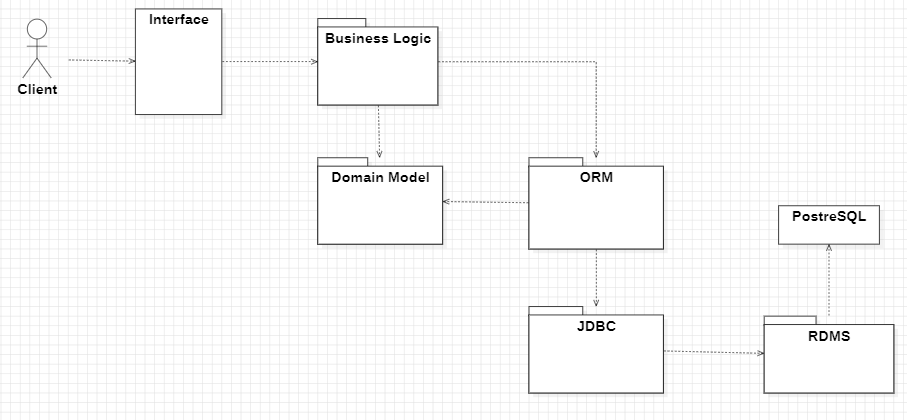
\includegraphics[scale=0.5]{Sp/StrutturaProgetto}
\par\medskip
Figura 1: Diagramma della struttura del progetto
\par\medskip
\end{center}
La struttura del progetto è stata divisa in tre parti:
\begin{itemize}
	\item \textbf{Business Logic}: contiene le classi che implementano la logica di business nel sistema.
	\item \textbf{Domain Model}: contiene le classi che rappresentano le entità del sistema.
	\item \textbf{DAO}: contiene le classi che permettono di gestire la comunicazione tra l'applicazione e il database andando a separare la logica per l'interazione con i dati dal resto dell'applicazione.
\end{itemize}
Infine per l'uso del software e l'interazione con il sistema è stata creata un'interfaccia a linea di comando (CLI).\\
Sono state utilizzate le seguenti piattaforme e software:
\begin{itemize}
\item \textbf{IntelliJ IDEA}: IDE per lo sviluppo in Java.
\item \textbf{StarUML}: software per la creazione di diagrammi UML.
\item \textbf{Draw.io}: software per la realizzazione di altri diagrammi (es: modello ER).
\item \textbf{PgAdmin}: software per la gestione del database PostgreSQL.
\item \textbf{GitHub}: piattaforma contenente il codice sorgente.
\item \textbf{Lunacy}: software per la realizzazione dei mockup.
\end{itemize}


\section{Progettazione}
\subsection{Use Case Diagram}

In questo progetto sono presenti 2 tipi di utenti: lo User e l'Admin. Nel diagramma sottostante vengono rappresentati i casi d'uso per i due tipi di utenti: 

\begin{center}
\includegraphics[scale=0.5]{usecases/UseCase1}
\includegraphics[scale=0.4]{usecases/UseCase2}\\
Figura 2: Use Case Diagram dello User e dell'Admin
\end{center}

\subsection{Use Case Template}
Sono di seguito alcuni template dei casi d'uso. In alcuni di essi sono presenti riferimenti a mockup presenti successivamente (sezione 2.3):

\begin{center}
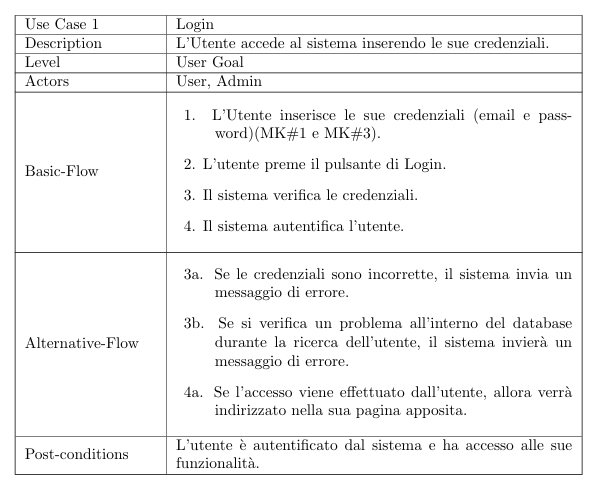
\includegraphics[scale=0.6]{templates/tabella1}
\par\medskip
Figura 3: Template che descrive il caso d'uso del login
\par\medskip
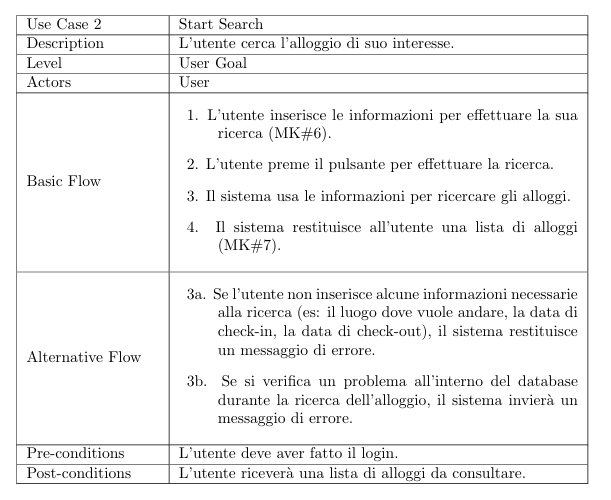
\includegraphics[scale=0.65]{templates/tabella2}
\par\medskip
Figura 4: Template che descrive il caso d'uso dello Start Research
\par\medskip
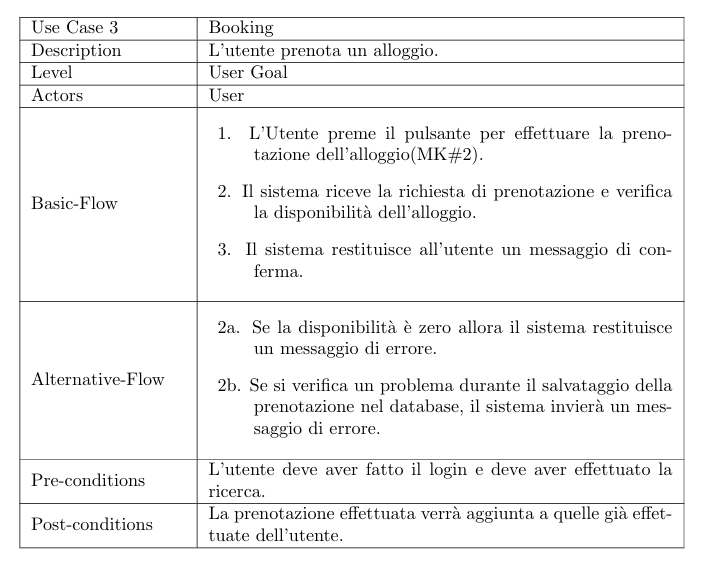
\includegraphics[scale=0.6]{templates/tabella3}
\par\medskip
Figura 5: Template che descrive il caso d'uso del Booking
\par\medskip
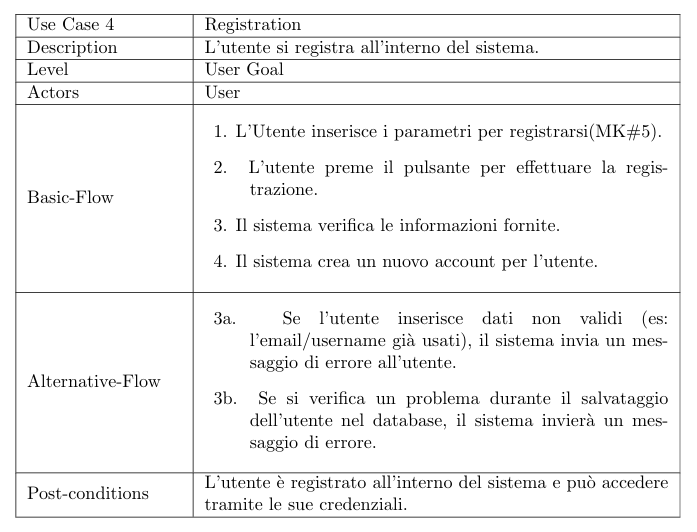
\includegraphics[scale=0.6]{templates/tabella4}
\par\medskip
Figura 6: Template che descrive il caso d'uso del Registration
\par\medskip
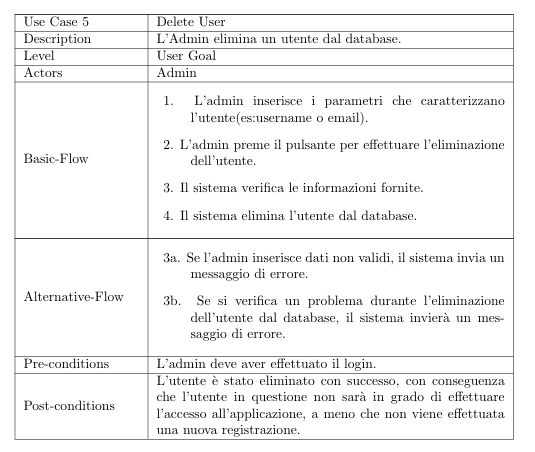
\includegraphics[scale=0.7]{templates/tabella5}
\par\medskip
Figura 7: Template che descrive il caso d'uso del Delete User
\par\medskip
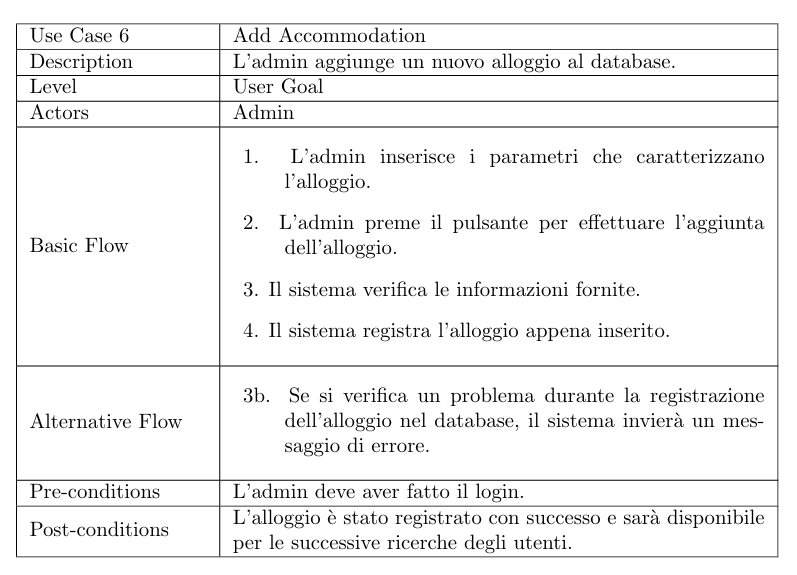
\includegraphics[scale=0.5]{templates/tabella6}
\par\medskip
Figura 8: Template che descrive il caso d'uso dell'Add Accomodation
\par\medskip
\end{center}


\subsection{Mockups}
Nella sezione in questione sono riportati alcuni mockup relativi ad una possibile interfaccia grafica per l'applicazione:
\begin{center}
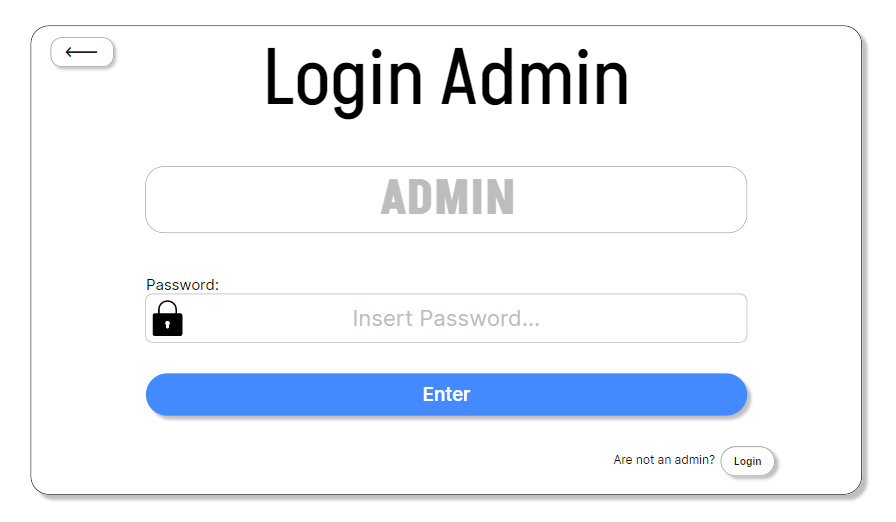
\includegraphics[scale=0.6]{Mockup/MockupAdminLogin}
\par\medskip
Figura 9: Mockup per il login effettuato da un admin - MK\#1 
\par\medskip
\par\medskip
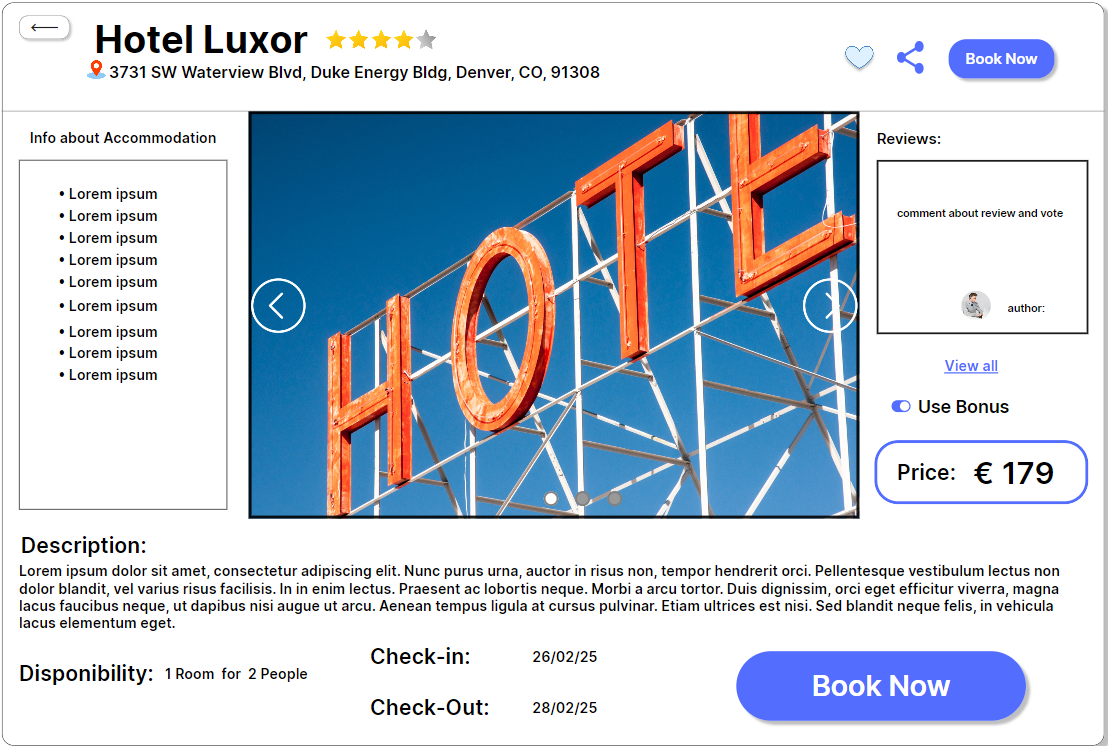
\includegraphics[scale=0.5]{Mockup/mockupBooking}
\par\medskip
\par\medskip
Figura 10: Mockup per mostrare in dettaglio un alloggio con la possibilità di prenotarlo - MK\#2
\par\medskip
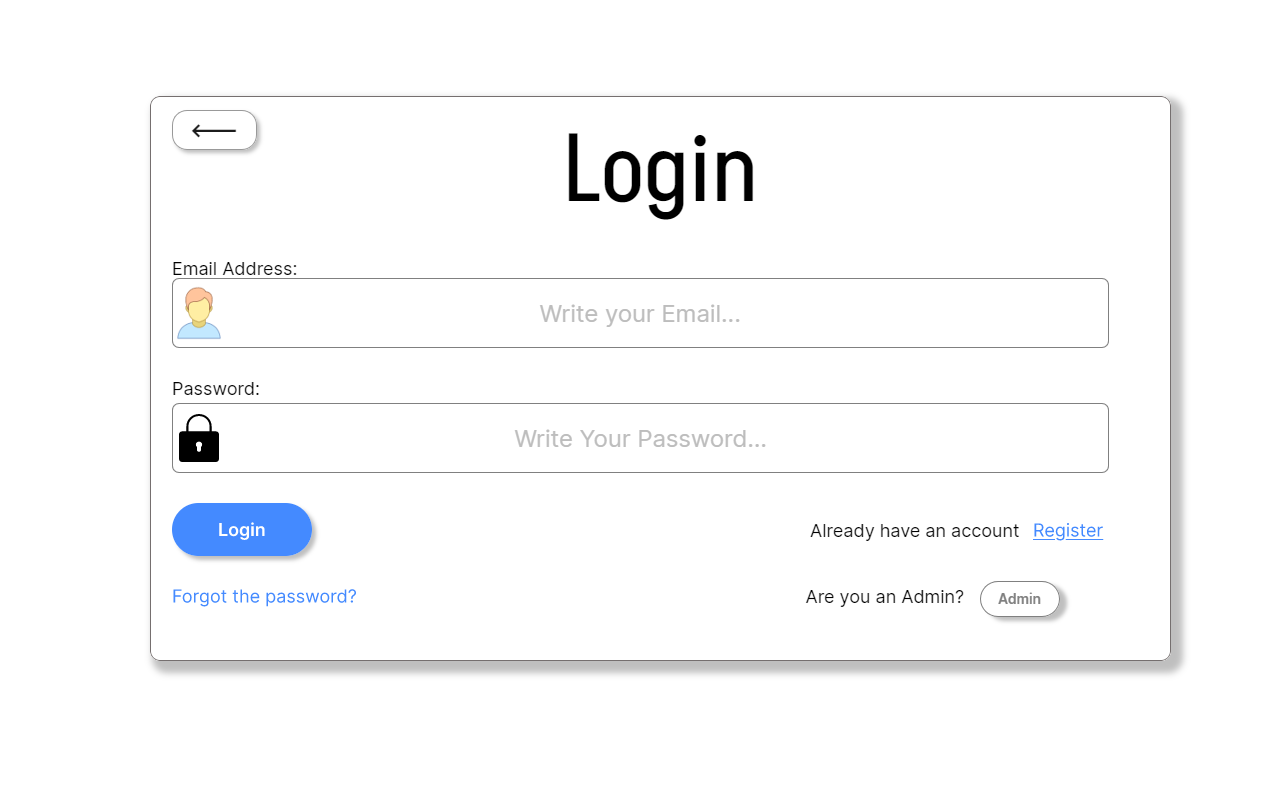
\includegraphics[scale=0.5]{Mockup/MockupLogin}
\par\medskip
Figura 11: Mockup per il login effettuato da un utente - MK\#3
\par\medskip
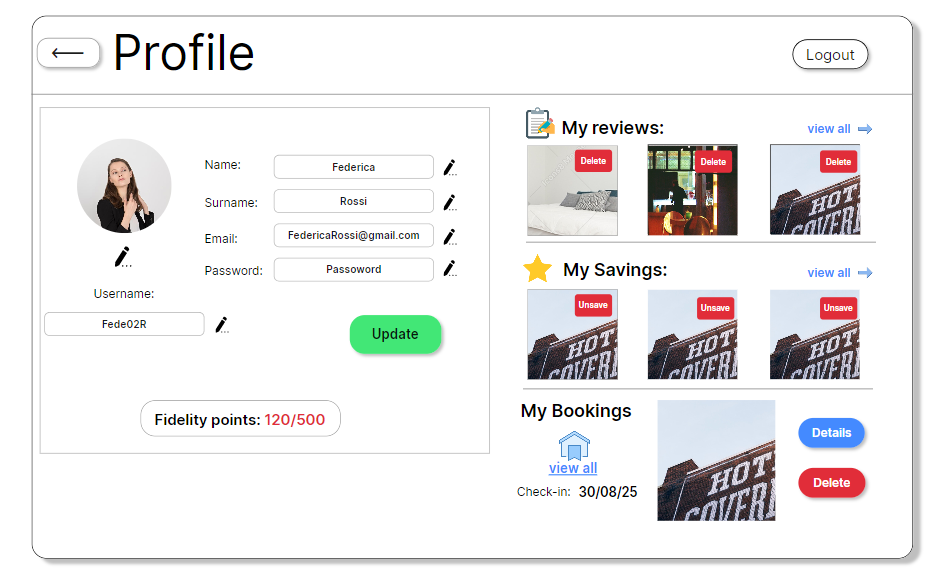
\includegraphics[scale=0.6]{Mockup/MockupProfile}
\par\medskip
Figura 12: Mockup per mostrare il profilo di un utente - MK\#4
\par\medskip
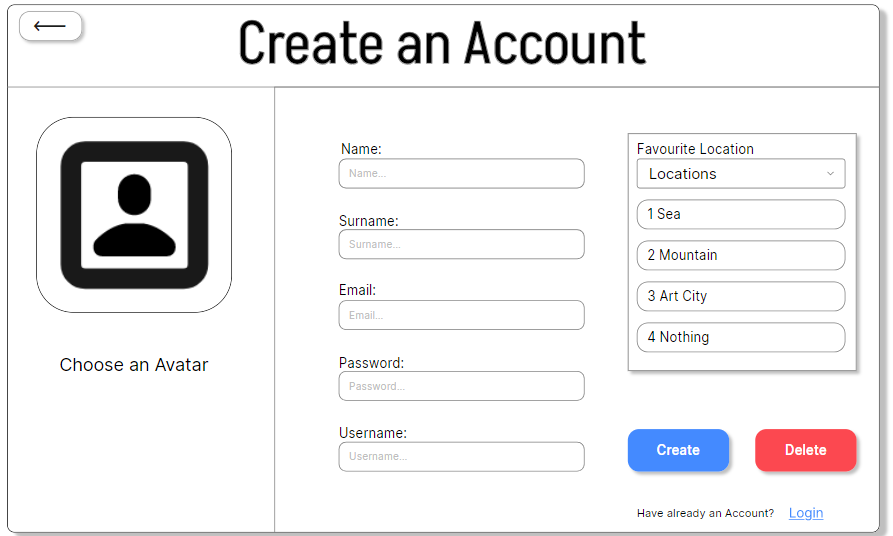
\includegraphics[scale=0.6]{Mockup/MockupRegister}
\par\medskip
\par\medskip
Figura 13: Mockup per creare un account - MK\#5
\par\medskip
\par\medskip
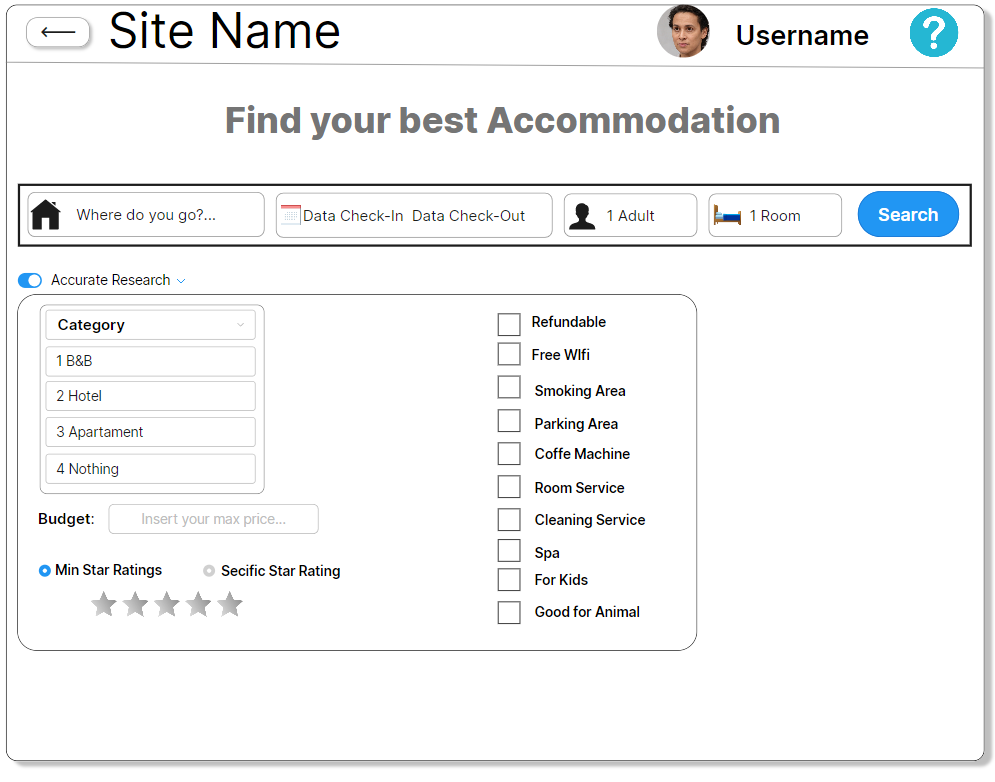
\includegraphics[scale=0.6]{Mockup/MockupResearch}
\par\medskip
Figura 14: Mockup per effettuare la ricerca attraverso i filtri - MK\#6
\par\medskip
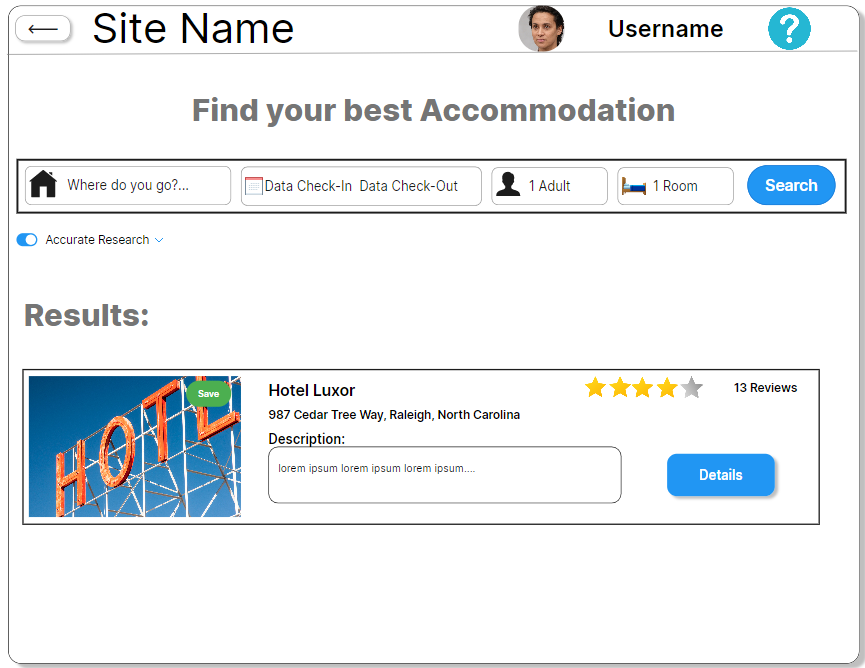
\includegraphics[scale=0.6]{Mockup/MockupResult}
\par\medskip
Figura 15: Mockup che mostra i risualtati di una ricerca - MK\#7
\par\medskip
\end{center}

\subsection{Class Diagram}
Come spiegato precedentemente, Il progetto è diviso in 3 package:
\begin{itemize}
\item \textbf{Business Logic}:è il package che contiene i controller, che sono 4: quello che gestisce l'accesso, la registrazione e l'eliminazione degli utenti (\textbf{UserController}), quello che gestisce il profilo dell'utente (\textbf{ProfileUserController}), quello che gestisce la logica dell'applicazione (ricerca,prenotazione,recensione) (\textbf{ResearchController}) e quello che gestisce le azioni che può effettuare l'Admin (\textbf{AdminController}). 
\item \textbf{Domain Model}: consiste nell’insieme di classi che rappresentano i concetti con cui interagisce l’applicazione: \textbf{RegisterUser}, \textbf{Review}, \textbf{Booking}, \textbf{Accommodation}, \textbf{SearchParameters}, \textbf{ReviewMapper}, \textbf{SearchParametersBuilder}.
\item \textbf{DAO}: è il package che si occupa di gestire la connessione con il database: \textbf{UserDAO}, \textbf{BookingDAO}, \textbf{PreferenceDAO}, \textbf{ReviewDAO}, \textbf{AccommodationDAO}, \textbf{DatabaseConnection}.
\end{itemize}
\begin{center}
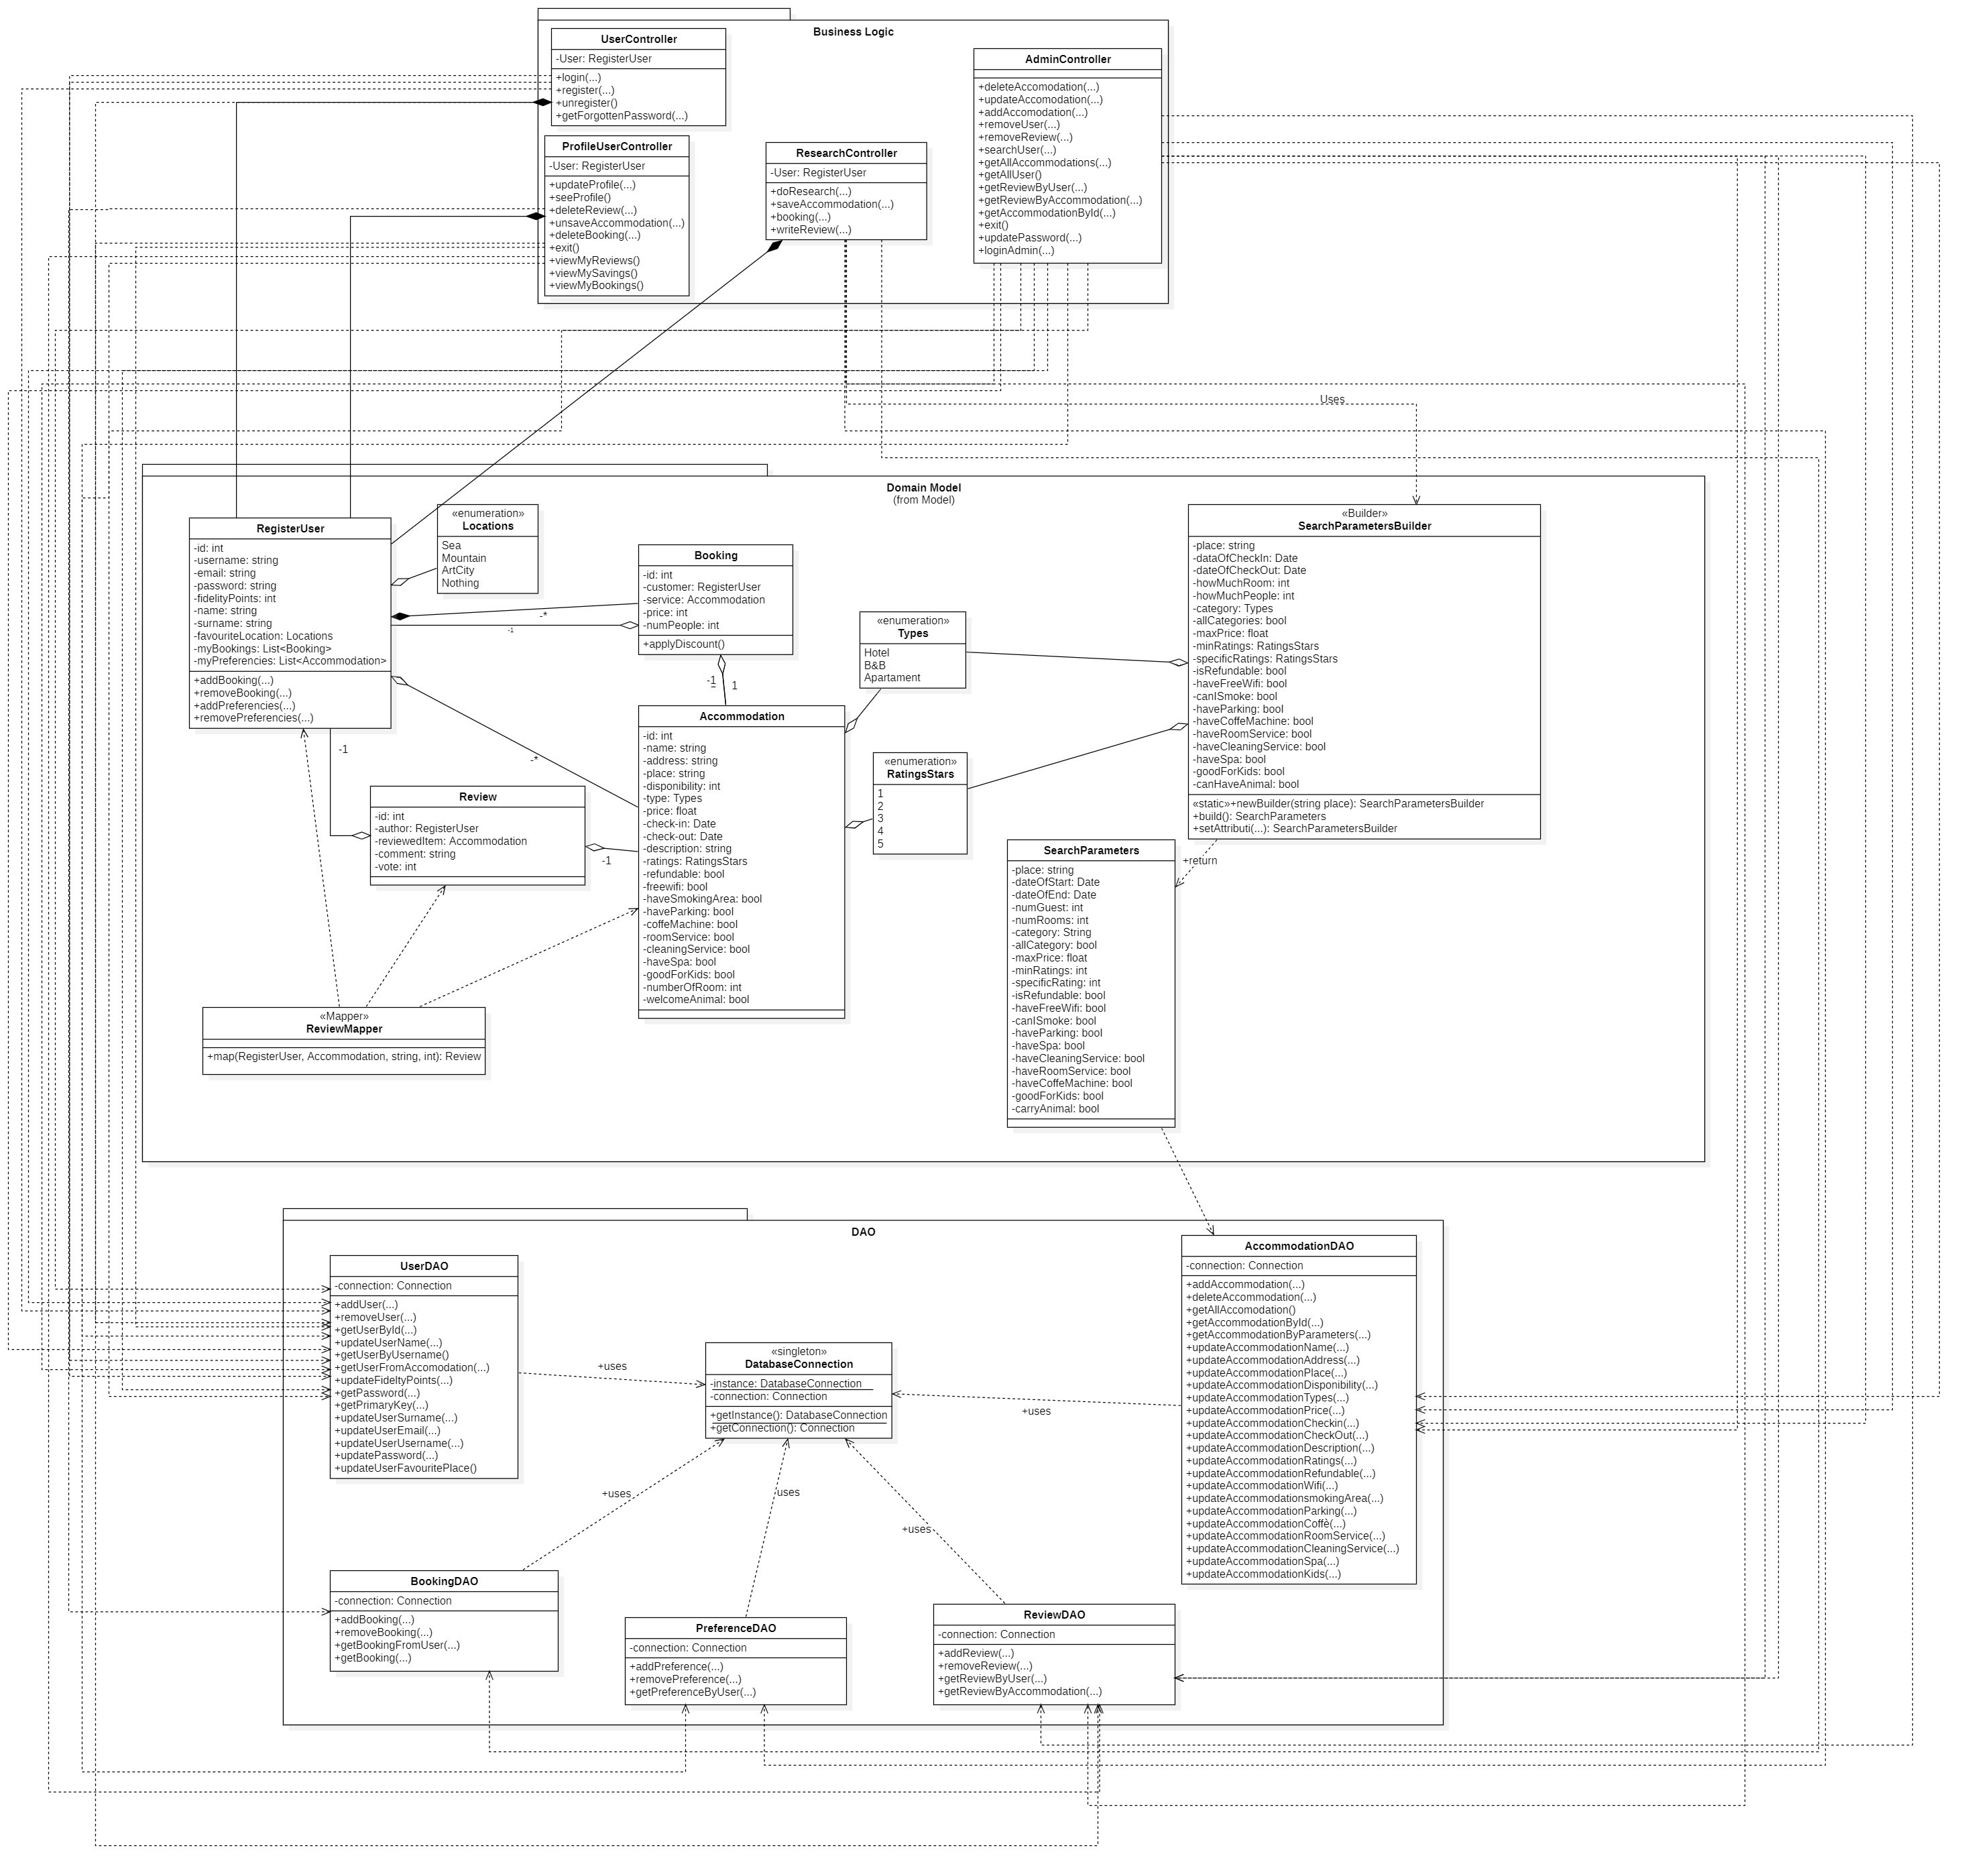
\includegraphics[scale=0.2]{uml/UML3}
\par\medskip
Figura 16: Mockup che mostra i risualtati di una ricerca - MK\#7
\par\medskip
\end{center}
\subsection{Design Patterns}
Nel progetto sono stati usati i seguenti design pattern:
\subsubsection{Singleton}

Lo scopo del Singleton è quello di creare una singola istanza di classe in tutto il sistema. Nel progetto è stato utilizzato per garantire che la connessione al database venisse effettuata una singola volta e per evitare conflitti tra connessioni.

\subsubsection{Mapper}

Lo scopo del Mapper è di semplificare il codice e renderlo più modulare, separando la logica di relazione degli oggetti dal resto dell'applicazione. Nel nostro progetto è stata implementata per creare la relazione tra utenti, recensioni e alloggi.

\subsubsection{Builder}

Il Builder separa la costruzione del suo oggetto dalla sua rappresentazione, rendendo la creazione della classe più flessibile, leggibile e facile da mantenere. Nel nostro progetto viene usato per creare la classe parametri di ricerca essendo che presenta tanti attributi, spesso opzionali, e consente una gestione più efficiente.

\subsubsection{DAO}

Il DAO (Data Access Object) è un design pattern che si occupa di separare le classi che si interfacciano al database dall'applicazione. Questo viene fatto
per poter meglio implementare il principio di singola responsabilità e aumenta
la mantenibilità del codice.

\subsection{ER Diagram e Relational Model}

Per il database e la sua gestione, è stato realizzato un ER Diagram (Figura 17), e il Relational Model derivato (Figura 18). Ci sono state delle scelte progettuali precise, in particolare quella riguardante l'entità \textbf{Alloggio}, dove per differenziare i tipi di alloggio è stato usato un'attributo al posto di una generalizzazione, dovuto al fatto che nel progetto si faranno uso di informazioni che sono a comune tra i vari alloggi, favorendo accessi più veloci ma a discapito di un notevole spreco di memoria e la presenza di valori nulli.\\
Alla fine sono state definite le seguenti tabelle (Figura 19):
\begin{itemize}
\item \textbf{User}: rappresenta l'entità \textbf{User}.
\item \textbf{Booking}: rappresenta l'entità \textbf{Booking}.
\item \textbf{Acccommodation}: rappresenta l'entità \textbf{Accommodation}.
\item \textbf{Review}: rappresenta la relazione \textbf{Review} che avviene tra l'entità \textbf{User} e l'entità \textbf{Accommodation}.
\item \textbf{Favourites}: rappresenta la relazione \textbf{Like} che avviene tra l'entità \textbf{User} e l'entità \textbf{Accommodation}.
\end{itemize}

\begin{center}
\par\medskip
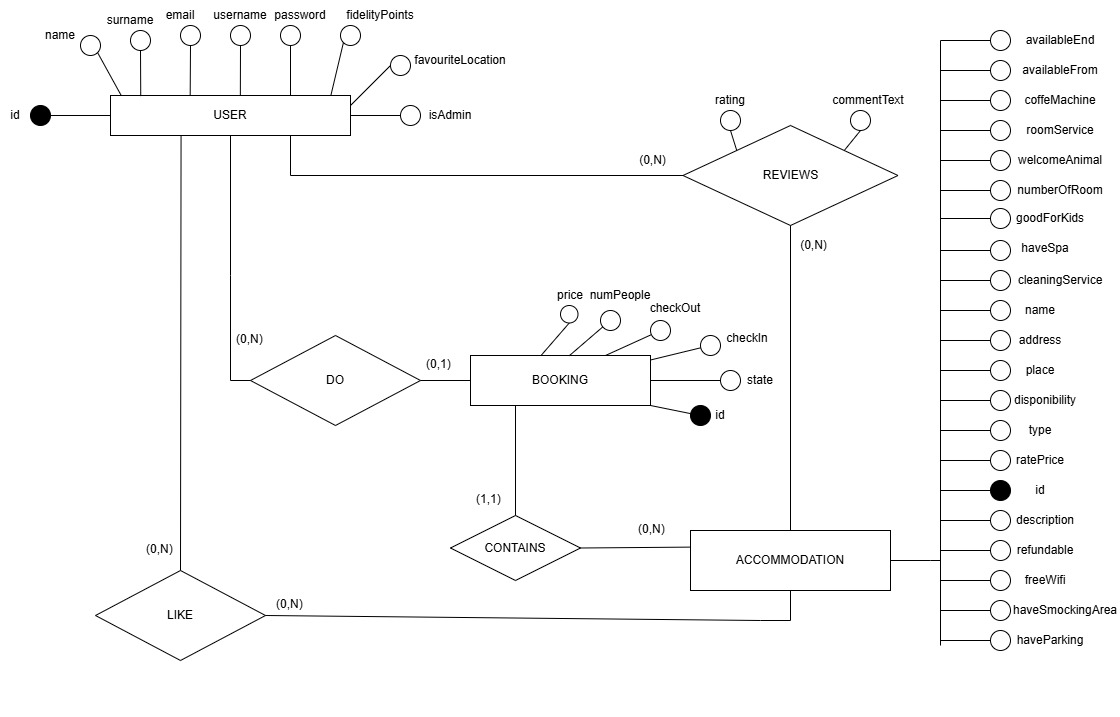
\includegraphics[scale=0.6]{ERImages/finalER}
\par\medskip
Figura 17: ER Diagram
\par\medskip
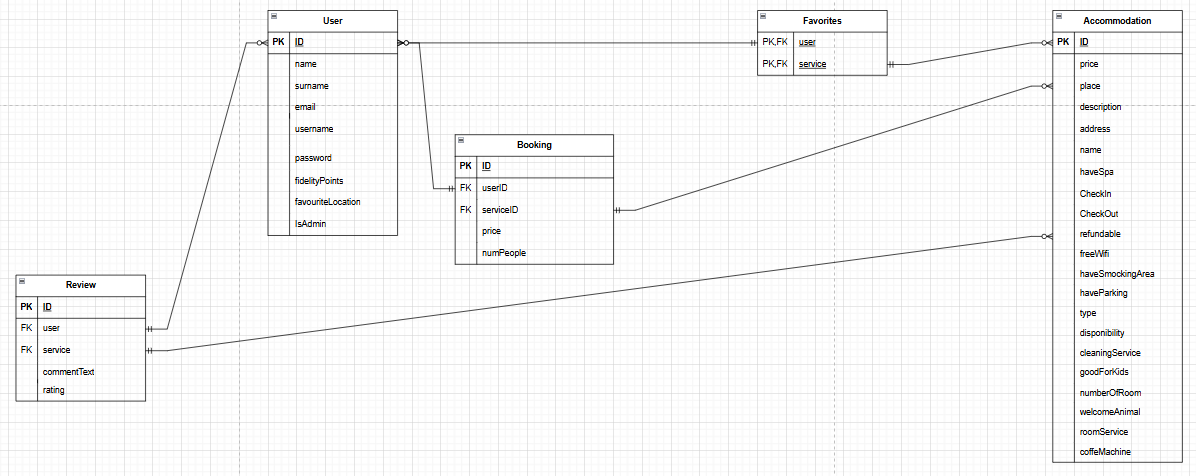
\includegraphics[scale=0.5]{ERImages/finaleTablesER}
\par\medskip
Figura 18: Tables of the database
\par\medskip
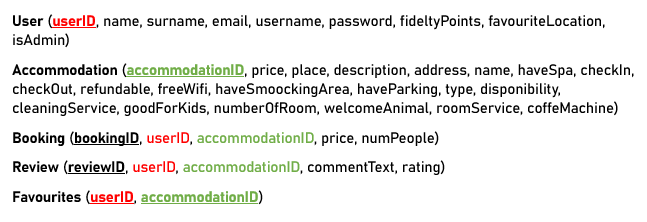
\includegraphics[scale=1]{ERImages/RelationalModel}
\par\medskip
Figura 19: Relation Model
\par\medskip
\end{center}

\section{Implementazione}
\subsection{Business Logic}

\`E il package che contiene i controller e che espone all'esterno le funzionalità dell'applicazione. \`E responsabilità dei controller gestire le dipendenze tra gli oggetti creati dai DAO.

\subsubsection{UserController}

\`E la classe che si occupa di implementare le funzionalità di un utente generico per l'accesso all'applicazione. Infatti presenta i metodi di login, di registrazione, cancellare l'utente in uso e un eventuale recupera password.

\subsubsection{ProfileController}

\`E la classe che si occupa di gestire le informazioni del profilo utente e dei servizi di cui ha usufruito (\textbf{deleteReview()}, \textbf{deleteBooking()}, \textbf{unsaveAccommodation()}, \textbf{viewMySavings()}, \textbf{viewMyReviews()}, \textbf{viewMyBookings()}).

\subsubsection{ResearchController}

\`E la classe che si occupa di fornire i metodi che implementano la logica dell'applicazione. Infatti, permette la ricerca in base a dei parametri (\textbf{doResearch()}) e sugli alloggi ricercati permette,a un utente registrato, di effettuare una prenotazione (\textbf{booking()}), salvarlo tra i preferiti (\textbf{saveAccomodation()}) e scrivere una recensione su quell'alloggio (\textbf{writeReview()}). Per funzionare, oltre ai collegamenti ai relativi DAO, questa classe usa il \textbf{SearchParametersBuilder} che si trova nel \textbf{Domain Model}.

\subsubsection{AdminController}

\`E la classe che si occupa di implementare le operazioni dell'admin, il quale può  leggere, modificare, cancellare e aggiungere alloggi, mentre può solo leggere e cancellare utenti e recensioni.
 
\subsection{Domain Model}

\`E il package che rappresenta il modello dei dati e implementa le classi che raffigurano le entità del sistema.

\subsubsection{RegisterUser}

Contiene le informazioni relative all'utente registrato. Gli attributi della classe sono: id (utilizzato come identificativo), username, email (unica all'interno dell'applicazione), password, nome, cognome, punti fedeltà (che si aggiornano ad ogni acquisto e raggiunta una certa soglia, permette di avere degli sconti), località preferita che indica un genere di esperienza che preferisce, la lista delle prenotazioni effettuate e la lista dei suoi alloggi preferiti. 

\subsubsection{Booking}

\`E la classe che rappresenta l'entità prenotazione, con tutte le informazioni relative ad essa. Possiede un id identificativo, l'acquirente, il servizio, per quante persone è la prenotazione e il prezzo.

\subsubsection{Accommodation}

\`E la classe che rappresenta l'entità alloggio e tiene conto dei suoi attributi. Molti dei suoi attributi non sono obbligatori, ma possono essere nulli perché dipendono dai servizi che offre l'alloggio. Ha un id (univoco), un nome, un indirizzo, un luogo, quante persone possono alloggiarci, tipo di alloggio (B\&B, appartamento e hotel), il prezzo, il check-in, il check-out, la descrizione di cosa offre, e diversi parametri aggiuntivi che non sono obbligatori (visualizzabili nelle figure precedenti).

\subsubsection{Review}

\`E la classe che rappresenta l'entità recensione. I campi sono id, autore, alloggio recensito, commento e il voto.

\subsubsection{ReviewMapper}

\`E una classe creata per mappare i dati della recensione, cioè per relazionare un utente registrato e un alloggio.

\subsubsection{SearchParametersBuilder e SearchParameters}

Queste classi implementano il design pattern Builder per la creazione dei parametri di ricerca. Il \textbf{SearchParametersBuilder} consente una creazione più facile da gestire e da estendere dei parametri di ricerca. Infatti il suo unico scopo è di creare la classe \textbf{SearchParameters} (devono possedere gli stessi attributi). Quest'ultima classe possiede solo gli attributi che poi serviranno alla ricerca all'interno del database. Gli attributi sono per la maggior parte uguali alla classe \textbf{Accommodation} (si possono visualizzare nell'UML visto precedentemente).

\subsection{DAO}

\`E il package che implementa l'omonimo design pattern descritto nella sezione 2.5.4. Le classi in questo package permettono alle classi presenti nella \textbf{Business Logic} di accedere ai vari dati di loro interesse.

\subsubsection{DatabaseConnection}

\`E la classe che si occupa di gestire la connessione al database per le altre classi DAO tramite il metodo \textbf{getConnection()}. Classe implementata usando il design pattern \textit{Singleton} per evitare conflitti tra connessioni.

\subsubsection{UserDAO}

\`E la classe che si occupa della gestione dei dati degli utenti. Questa classe contiene molti metodi, offrendo la possibilità di aggiungere nuovi utenti e di rimuovere quelli già presenti nel database (rispettivamente \textbf{addUser()} e \textbf{removeUser()}), la possibilità di recuperare un utente tramite l'id identificativo (\textbf{getUserById()}) oppure tramite lo username (\textbf{getUserByUsername()}) o anche in altri modi.Infine la classe presenta i metodi che permettono di aggiornare i dati personali di un utente.

\subsubsection{BookingDAO}

\`E la classe che si occupa della gestione dei dati che riguardano le prenotazioni effettuate dagli utenti. La classe mette a disposizione metodi che permetto di aggiungere o rimuovere delle prenotazioni (rispettivamente \textbf{addBooking()} e \textbf{removeBooking()}), di visualizzare le prenotazioni fatte da uno specifico utente (\textbf{getBookingFromUser()}) o vederle tutte (quest'ultima utilizzata da un admin per effettuare dei controlli e modifiche se fosse necessario).

\subsubsection{PreferenceDAO}

\`E la classe che si occupa della gestione dei dati che riguardano le liste di alloggi preferiti dagli utenti, i quali posso essere visionati senza dover fare una nuova ricerca. Questa classe contiene i metodi che permettono di aggiungere un nuovo alloggio tra i preferiti (\textbf{addPreference()}), di rimuovere un alloggio tra i preferiti (\textbf{removePreference()}) e di visualizzare gli alloggi preferiti di uno specifico utente (\textbf{getPreferenceByUser()}). 

\subsubsection{ReviewDAO}

\`E la classe che si occupa della gestione delle recensioni scritte sugli alloggi da parte degli utenti. La classe contiene i metodi che permettono di aggiungere nuove recensioni (\textbf{addReview()}), di rimuovere le recensioni dall'applicazione (\textbf{removeReview()}), e di visualizzare le recensioni scritte da uno specifico utente (\textbf{getReviewByUser()}) o visualizzare le tutte le recensioni scritte su uno specifico alloggio (\textbf{getReviewByAccommodation()}). 

\subsubsection{AccommodationDAO}

\`E la classe che si occupa della gestione dei dati degli alloggi. questa classe presenta molti metodi, permettendo di aggiungere nuovi alloggi (\textbf{addAccommodation()}), di rimuovere gli alloggi già presenti (\textbf{deleteAccommodation()}), di visualizzare tutti gli alloggi (\textbf{getAllAccommodation()}), di visualizzare uno nello specifico tramite il suo identificativo (\textbf{getAccommodationById()}, questo metodo è molto utile per la gestione degli alloggi da parte dell'admin) e di visualizzare gli alloggi che vengono ricercati tramite l'uso dei filtri (\textbf{getAccommodationByParameters()}). Infine sono presenti i metodi che permettono di aggiornare i dati di un alloggio. 


\end{document}
